%\input epsf
\documentclass[12pt]{article}
\newtheorem{theorem}{Theorem}
\usepackage{graphicx}
\usepackage{amsmath}
\usepackage{cite}
\usepackage{amsfonts} \usepackage{amssymb}
%\bibliographystyle{siam}
\bibliographystyle{plain}
\pagestyle{myheadings}
%\setcounter{secnumdepth}{2}


\renewcommand{\theequation}{\thesection.\arabic{equation}}
\newcommand{\pdiff}[2]{\frac{\partial #1}{\partial #2}}
\newcommand{\pdiffsec}[2]{\frac{\partial^2 #1}{\partial #2}^2}
\newcommand{\matder}[2]{\frac{D^#1 #2}{Dt}}

\def\bnab{\mbox{\boldmath$\nabla$}}
\def\e{\varepsilon}
\def\eps{\epsilon}
\renewcommand\l{\ell}
\def\QED{{\ \vbox{\hrule\hbox{\vrule height1.3ex\hskip0.8ex\vrule}\hrule}}\par}
\def\ds{\displaystyle}
\def\b{\beta}


\begin{document}

\section{Stability Analysis}

\begin{eqnarray}\label{eq:VPIDE_System}
% \nonumber to remove numbering (before each equation)
\nonumber
  \dot{\e^\l} &=& (1-\e^\l)\bnab\cdot\left(D(\e^\l)\bnab\e^\l\right) + \mu(1-\e^\l)\left[\Delta\left(\e^\l - \e^{-\lambda t}\e^\l_0\right) - \lambda v(t)\right] \\
  \dot{v} &=& \Delta \e^\l-\lambda v,
\end{eqnarray}

Stability of numerical schemes for time-dependent problems depend on the eigenvalues of the differentiation matrices. Trefethen et. al. and Fornberg \cite{InstSpecMeth,FornbergText} show that after a certain size the eigenvalues of the second-order differentiation matrix in rectangular coordinates begin to grow like $\mathcal{O}(N^4)$ instead of $\mathcal{O}(N^2)$. Consequently this instability limits the number of points used in the approximation. This limitation can be problematic if one is using a Chebyshev collocation method to build the differentiation matrix. Recall that Chebyshev nodes are nearly equispaced in the interior of the interval with spacing $\mathcal{O}(\frac{1}{N})$ but cluster near the boundary with spacing roughly $\mathcal{O}(\frac{1}{N^2})$. So one must trade-off resolution in the interior for stability in the approximation for instance.

This problem is mitigated slightly for the polar Laplacian. In constructing the polar Laplacian differentiation matrices we could simply transform the radial interval, $[0,1]$, to $[-1,1]$ via $r' = 2r-1$ and construct the spectral differentiation matrix using an appropriate choice of orthogonal polynomial. This transformation has a couple of drawbacks since the points are clustered near the boundary and the origin. First, if the solution is smooth near the origin (in the interior of the disc), then this clustering is numerically inefficient; points are clustered in a region where it is not needed. Second, care must be taken near the origin with respect to numerical stability when applying the Laplacian in polar coordinates,
\begin{equation}\label{eq:polar_Laplacian}
\pdiffsec{(\cdot)}{r} +\frac{1}{r}\pdiff{(\cdot)}{r}+\frac{1}{r^2}\pdiffsec{(\cdot)}{\theta}.
\end{equation}

Clustering increases the size of the weights in the difference approximation and hence increases the size of the matrix entries where the clustering applies, near the corners of the differentiation matrix, see Figure~\ref{fig:weights_evs}(a). Therefore clustering points near the origin may result in prohibitively small time steps because the large weights imply large eigenvalues and the $\frac{1}{r}$ term in the polar Laplacian implies an additional increase in the size of the weights. So instead of transforming the points we proceed as in \cite{FornbergPSPolar, FornbergText,TrefethenMATLAB} and construct the polar Laplacian on $[-1,1]$ where half the points will be discarded by using symmetry. The result will be a discrete Laplacian matrix that operates over the radial interval, $[0,1]$ with $\mathcal{O}(\frac{1}{N})$ spacing near the origin and $\mathcal{O}(\frac{1}{N^2})$ clustering near the right boundary. Figure~\ref{fig:weights_evs}(b) reveals that the weights increase only at the right boundary of the interval with no clustering near the origin thus mitigating the impact of the $\frac{1}{r}$ term. We will call this latter construction the \emph{symmetric construction} while the former we will refer to as a consequence of \emph{interval shifting}. Figure~\ref{fig:weights_evs}(c) reveals that the symmetric construction exhibits preferable behavior with respect to the magnitudes of the eigenvalues.

\begin{figure}
\hfill
\begin{minipage}[H]{6.5cm}
\begin{center}
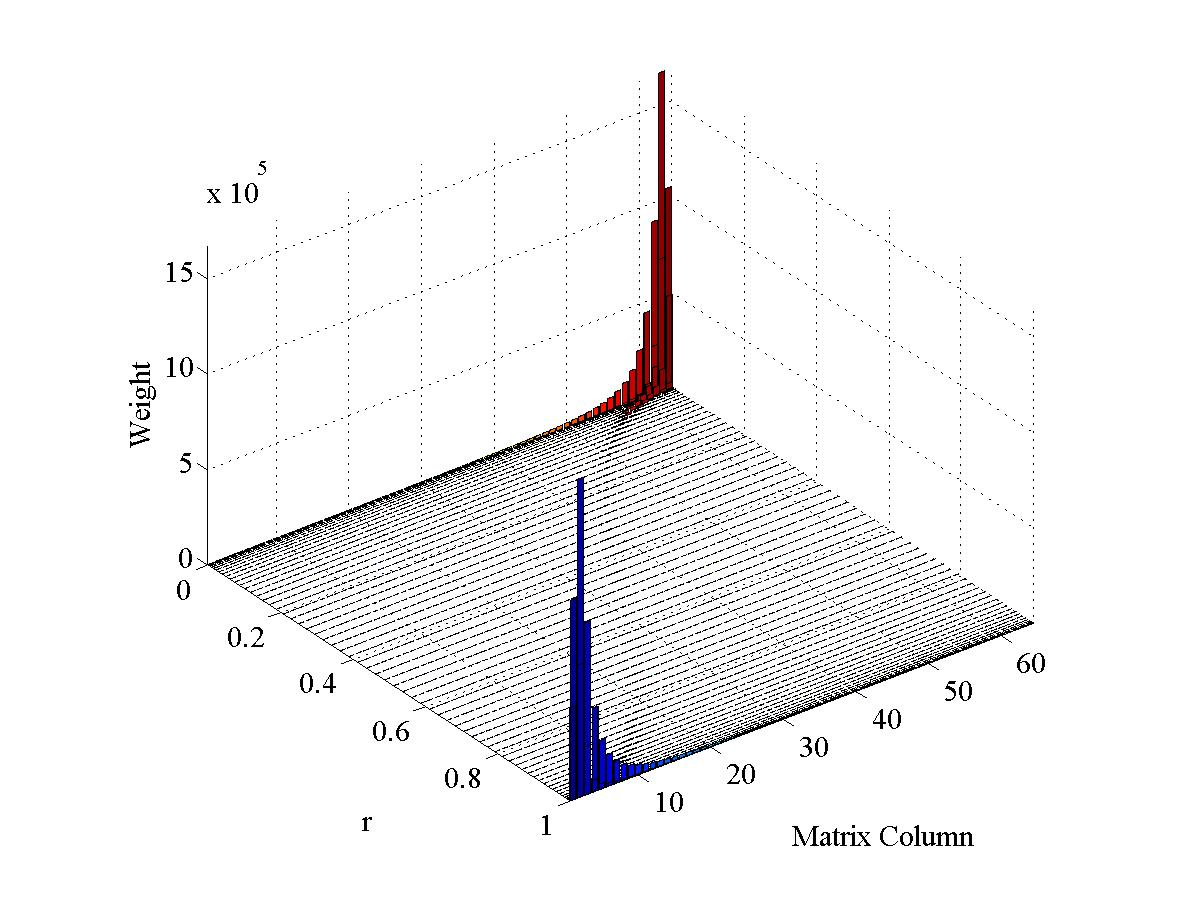
\includegraphics[width=6cm,clip]{20090806_Weights_ShiftedDM}
\end{center}
\begin{center}
(a)
\end{center}
\end{minipage}
\hfill
\begin{minipage}[H]{6.5cm}
\begin{center}
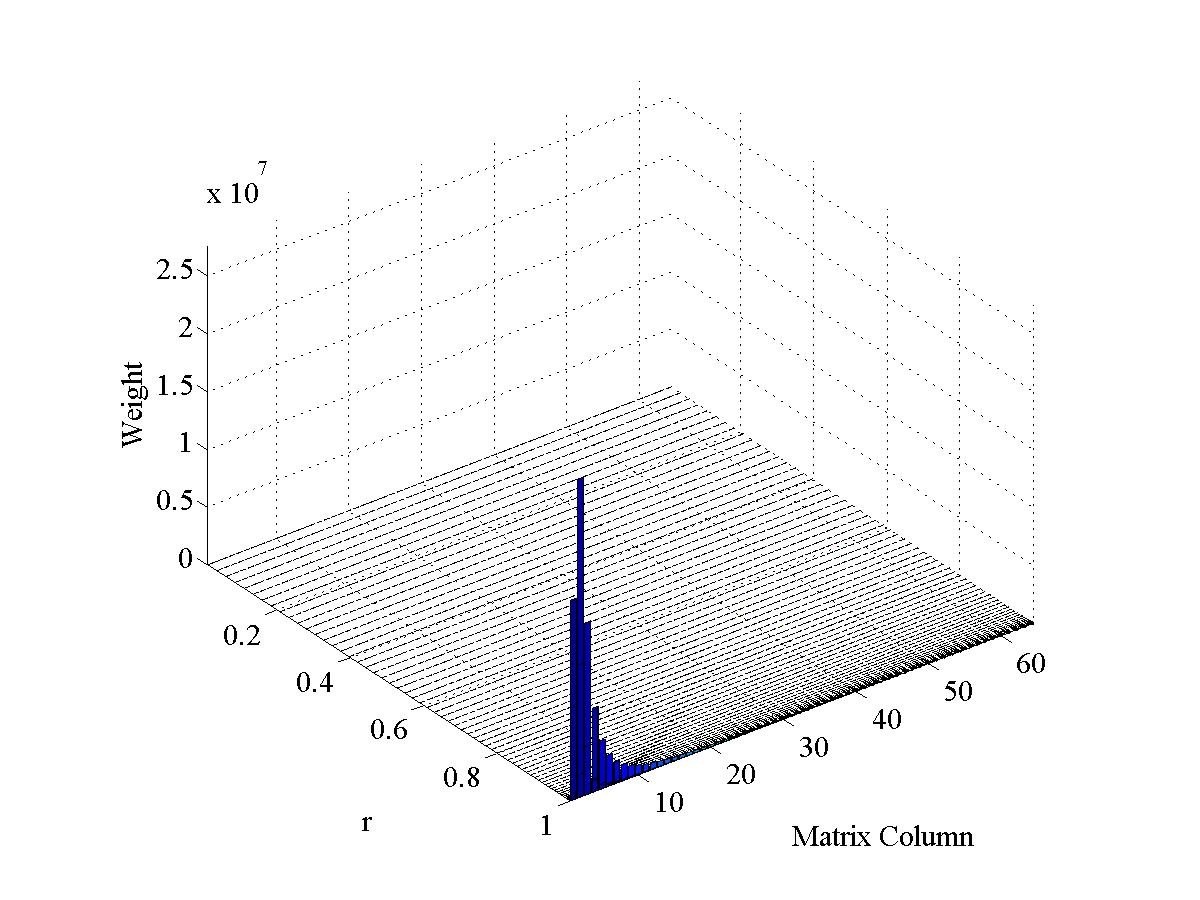
\includegraphics[width=6cm,clip]{20090806_Weights_TrefFornDM}
\end{center}
\begin{center}
(b)
\end{center}
\end{minipage}
\hfill
\begin{minipage}[H]{6.5cm}
\begin{center}
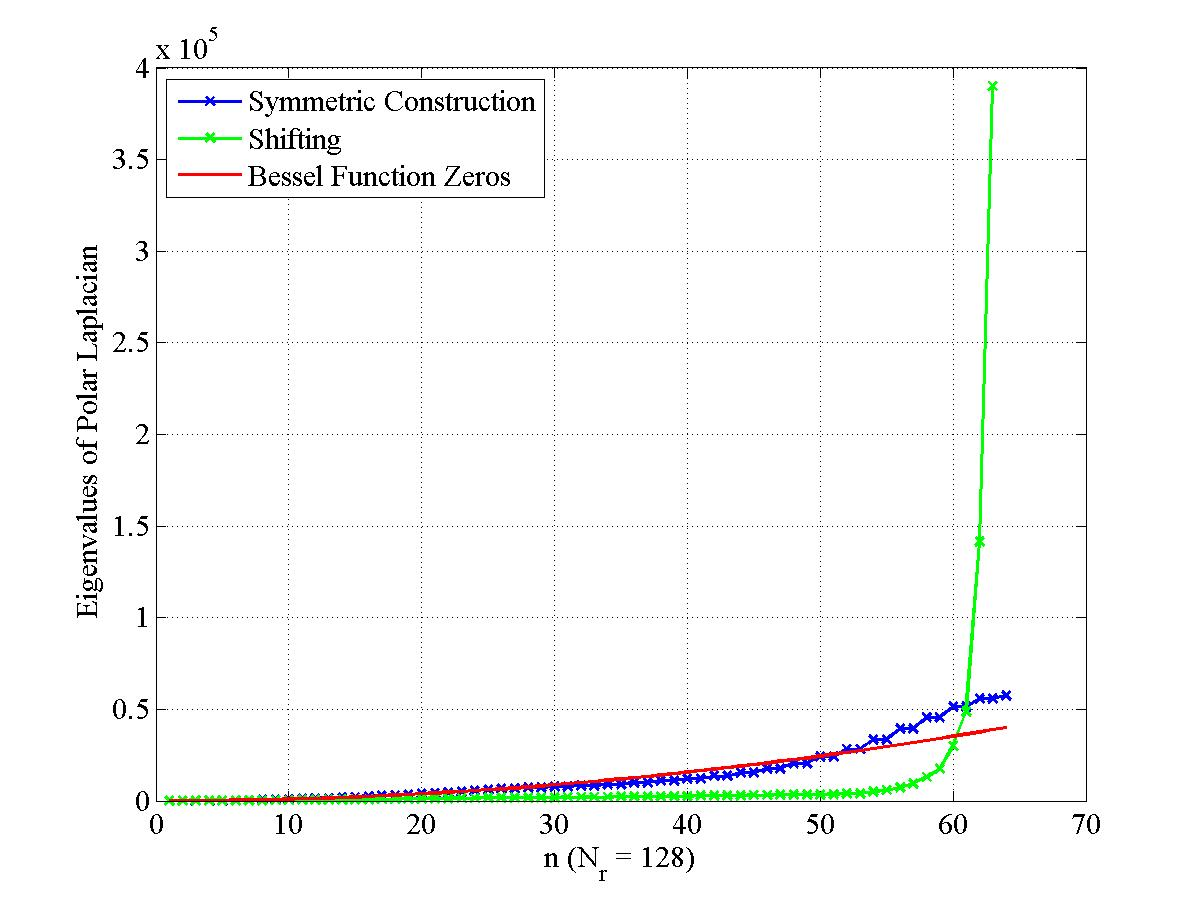
\includegraphics[width=6cm,clip]{20090806_evs_BesselZerosVsNumEvs3way}
\end{center}
\begin{center}
(c)
\end{center}
\end{minipage}
\caption{Differentiation matrix weights using (a) the symmetric construction and (b) the interval shift. The weights grow as the points cluster. (c) Eigenvalues of the respective differentiation matrices versus $\beta$ where $J_0(\beta)=0$, the zeros of the Bessel function of order zero (eigenvalues of the Polar Laplacian).}\label{fig:weights_evs}
\end{figure}

The problem we are solving has radial and angular symmetry so we will neglect that angular component of $\Delta$ for the remainder of this analysis. Using the symmetric construction we conducted a numerical experiment testing the stability of the RK4 scheme for increasing the matrix sizes. Differentiation matrices of sizes $N_r = 32, 34, \ldots, 62, 64$ were constructed and a test case was run, $\mu = 1e-004$ and $\lambda = 1e-006$, for step-sizes, $\Delta t = 1e-005, 2e-005, \ldots, 9e-005, 1e-004$ over the time interval $[0, 0.1]$; the test case was selected for its benign stability properties, as we will see below, stability is impacted by $\mu$ and $\lambda$. We then selected the maximum time-step that maintained stability. Results of this experiment are shown in Figure~\ref{fig:Delta_t_Vs_Nr}.

\begin{figure}
\begin{center}
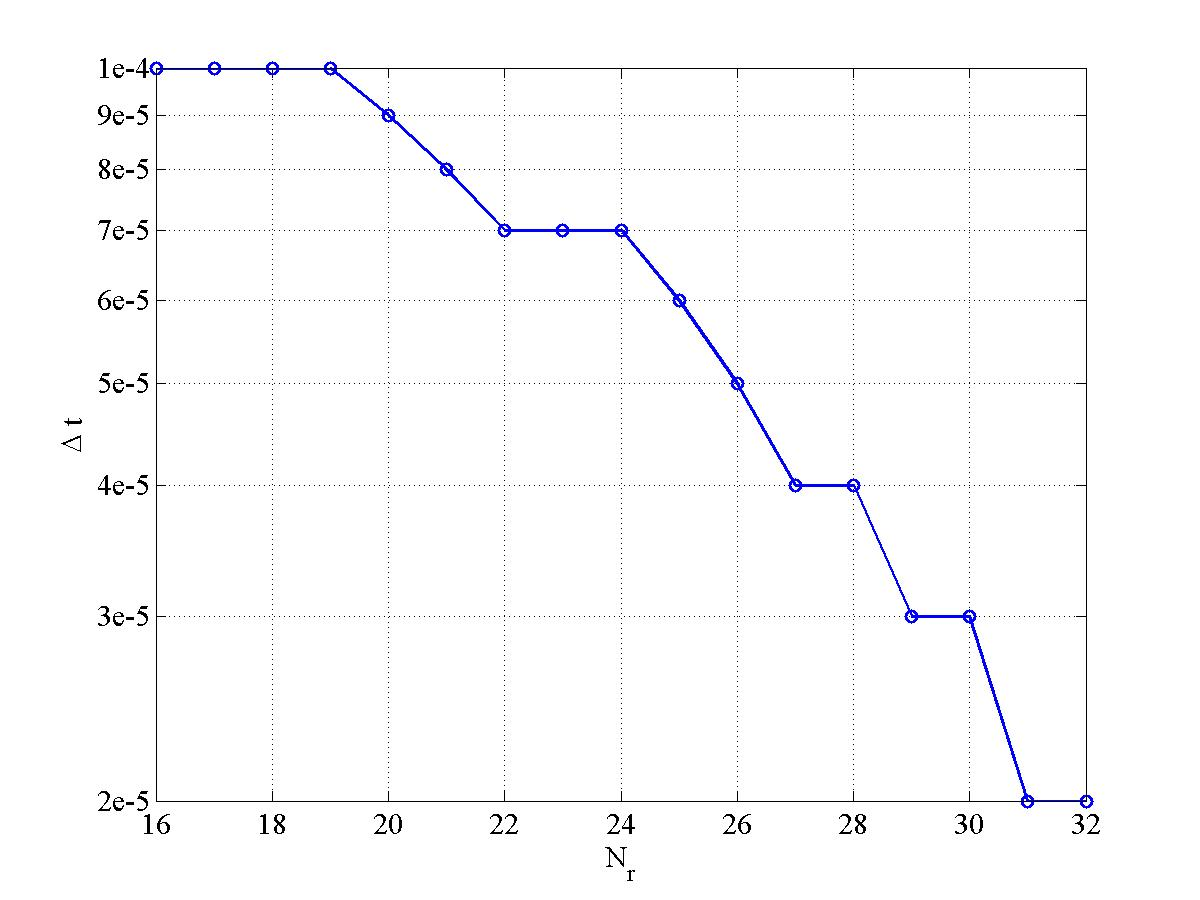
\includegraphics[width=8.5cm,clip]{20090805_Delta_t_Vs_Nr_stability}
\end{center}
\caption{Maximum time-step, $\Delta t$, maintaining stability using the RK4 time-marching scheme versus differentiation matrix size, $N_r$. The test case used $\mu = 1e-004$ and $\lambda = 1e-006$.}\label{fig:Delta_t_Vs_Nr}
\end{figure}


In the case that $\mu$ is nonzero, system (\ref{eq:VPIDE_System}) can be written as the matrix equation,
\begin{align*}
\begin{bmatrix}
\dot{\e^\l} \\
\dot{v}
\end{bmatrix} =
\begin{bmatrix}
\mu\Delta & -\mu\lambda\mbox{I}\\
\Delta & -\lambda\mbox{I}
\end{bmatrix}
\begin{bmatrix}
\e^l\\
v
\end{bmatrix}+N(\e^\l,t)
\end{align*}
where
\[
N(\e^\l,t) = (1-\e^\l)\bnab\cdot\left(D(\e^\l)\bnab\e^\l\right) - \mu\e^\l\Delta\left(\e^\l - \lambda v\right) -\mu e^{-\lambda t}(1-\e^\l)\Delta\e^\l_0.
\]

Now the VPIDE has been divided into linear and nonlinear parts. Let $\mathcal{L}$ define the linear part,
\begin{align*}
    \mathcal{L}=\begin{bmatrix}\mu\Delta & -\mu\lambda\mbox{I}\\
\Delta & -\lambda\mbox{I}\end{bmatrix},
\end{align*}
and now we can see the impact of $\mu$ and $\lambda$ on the stability of the RK4 time-stepper. The eigenvalues of the radial polar-Laplacian, $\Delta$, are $\b_m^2$ where $J_m(\b_m)=0$, the $m^{th}$-order Bessel function of the first kind (the eigenfunctions, $J_m(\b_m r)$, of $\Delta$). Since we know the eigenvalues of $\Delta$, it is easy to show that the non-zero eigenvalues of $\mathcal{L}$ are $\mu\b_m^2-\lambda$. Notice that in the case $\lambda=0$ the spectrum of $\mathcal{L}$ is equal to the spectrum of the sub-block $\mu\Delta$, $\Lambda(\mathcal{L})=\Lambda(\mu\Delta)$.

\bibliography{MyBiBTeX}
\bibliographystyle{plain}

\end{document}